\exercisesheader{}

% 25

\eoce{\qt{Side effects of Avandia\label{randomization_avandia}} Rosiglitazone is the 
active ingredient in the controversial type~2 diabetes medicine Avandia and has 
been linked to an increased risk of serious cardiovascular problems such as 
stroke, heart failure, and death. A common alternative treatment is pioglitazone, 
the active ingredient in a diabetes medicine called Actos. In a nationwide 
retrospective observational study of 227,571 Medicare beneficiaries aged  
65 years or older, it was found that 2,593 of the 67,593 patients using 
rosiglitazone and 5,386 of the 159,978 using pioglitazone had serious 
cardiovascular problems. These data are summarized in the contingency 
table below. \footfullcite{Graham:2010}
\begin{center}
\begin{tabular}{ll  cc c} 
                                &   & \multicolumn{2}{c}{\textit{Cardiovascular problems}} \\
\cline{3-4} 
                                    &               & Yes   & No        & Total \\
\cline{2-5}
\multirow{2}{*}{\textit{Treatment}} & Rosiglitazone & 2,593 & 65,000    & 67,593 \\
                                    & Pioglitazone  & 5,386 & 154,592   & 159,978 \\
\cline{2-5}
                                    & Total         & 7,979 & 219,592   & 227,571
\end{tabular}
\end{center}
\begin{parts}
\item Determine if each of the following statements is true or false. If false, explain why. \textit{Be careful:} The reasoning may be wrong even if the statement's conclusion is correct. In such cases, the statement should be considered false.
\begin{subparts}
\item Since more patients on pioglitazone had cardiovascular problems (5,386 vs. 2,593), we can conclude that the rate of cardiovascular problems for those on a pioglitazone treatment is higher.
\item The data suggest that diabetic patients who are taking rosiglitazone are more likely to have cardiovascular problems since the rate of incidence was (2,593 / 67,593 = 0.038) 3.8\% for patients on this treatment, while it was only (5,386 / 159,978 = 0.034) 3.4\% for patients on pioglitazone.
\item The fact that the rate of incidence is higher for the rosiglitazone group proves that rosiglitazone causes serious cardiovascular problems.
\item Based on the information provided so far, we cannot tell if the difference between the rates of incidences is due to a relationship between the two variables or due to chance.
\end{subparts}
\item What proportion of all patients had cardiovascular problems?
\item If the type of treatment and having cardiovascular problems were independent, about how many patients in the rosiglitazone group would we expect to have had cardiovascular problems?
\item We can investigate the relationship between outcome and treatment in this study using a randomization technique.  While in reality we would carry out the simulations required for randomization using statistical software, suppose we actually simulate using index cards. In order to simulate from the independence model, which states that the outcomes were independent of the treatment, we write whether or not each patient had a cardiovascular problem on cards, shuffled all the cards together, then deal them into two groups of size 67,593 and 159,978. We repeat this simulation 1,000 times and each time record the number of people in the rosiglitazone group who had cardiovascular problems. Use the relative frequency histogram of these counts to answer (i)-(iii).
\end{parts}
\begin{minipage}[c]{0.5\textwidth}
\begin{subparts}
\item What are the claims being tested?
\item Compared to the number calculated in part (b), which would provide more support for the alternative hypothesis,  \textit{more} or \textit{fewer} patients with cardiovascular problems in the rosiglitazone group?
\item What do the simulation results suggest about the relationship between taking rosiglitazone and having cardiovascular problems in diabetic patients?
\end{subparts}
\end{minipage}
\begin{minipage}[c]{0.5\textwidth}
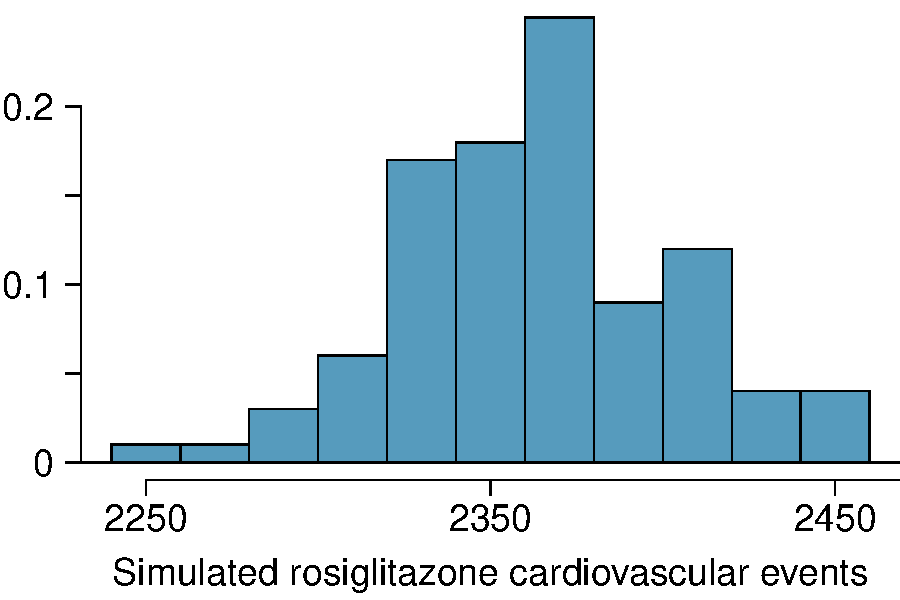
\includegraphics[width = \textwidth]{ch_summarizing_data/figures/eoce/randomization_avandia/randomization_avandia.pdf} \\
\end{minipage}
}{}

% 26

\eoce{\qt{Heart transplants\label{randomization_heart_transplants}} The Stanford 
University Heart Transplant Study was conducted to determine whether an 
experimental heart transplant program increased lifespan. Each patient 
entering the program was designated an official heart transplant candidate, 
meaning that he was gravely ill and would most likely benefit from a new heart. 
Some patients got a transplant and some did not. The variable \texttt{transplant} 
indicates which group the patients were in; patients in the treatment group got a 
transplant and those in the control group did not. Of the 34 patients in the 
control group, 30 died. Of the 69 people in the treatment group, 45 died. Another 
variable called \texttt{survived} was used to indicate whether or not the patient 
was alive at the end of the study. \footfullcite{Turnbull+Brown+Hu:1974}
\begin{center}
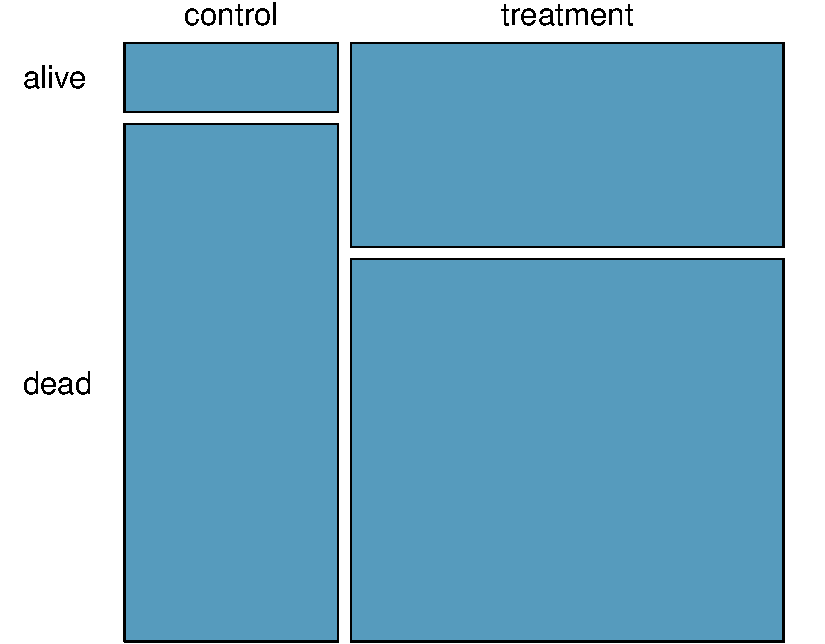
\includegraphics[width= 0.48\textwidth]{ch_summarizing_data/figures/eoce/randomization_heart_transplants/randomization_heart_transplants_mosaic.pdf}
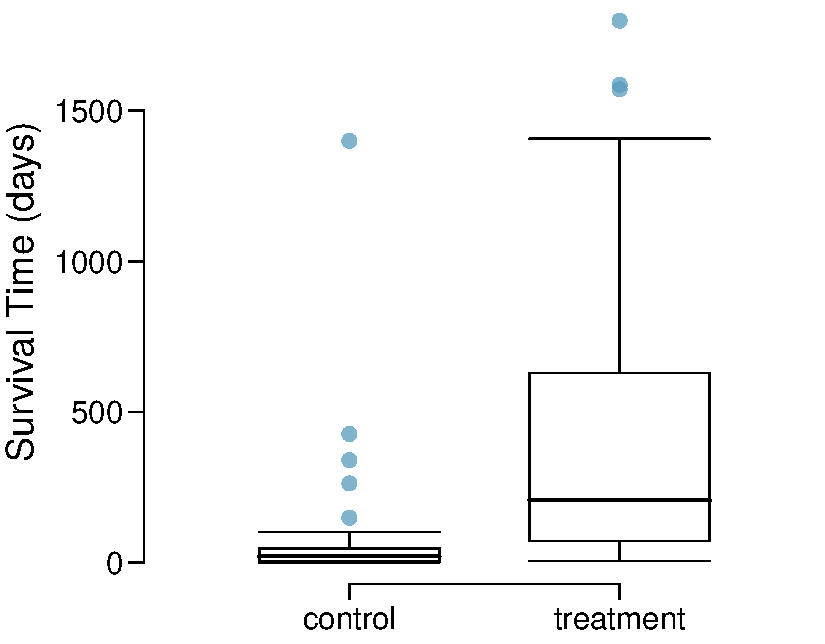
\includegraphics[width= 0.48\textwidth]{ch_summarizing_data/figures/eoce/randomization_heart_transplants/randomization_heart_transplants_box.pdf}
\end{center}
\begin{parts}
\item Based on the mosaic plot, is survival independent of whether or not the 
patient got a transplant? Explain your reasoning.
\item What do the box plots below suggest about the efficacy (effectiveness) of the heart transplant treatment.
\item What proportion of patients in the treatment group and what proportion of 
patients in the control group died?
\item One approach for investigating whether or not the treatment is effective 
is to use a randomization technique.
\begin{subparts}
\item What are the claims being tested?
\item The paragraph below describes the set up for such approach, if we were 
to do it without using statistical software. Fill in the blanks with a number 
or phrase, whichever is appropriate.
\begin{adjustwidth}{2em}{2em}
We write \textit{alive} on \rule{2cm}{0.5pt} cards representing patients who were 
alive at the end of the study, and \textit{dead} on \rule{2cm}{0.5pt} cards 
representing patients who were not. Then, we shuffle these cards and split them 
into two groups: one group of size \rule{2cm}{0.5pt} representing treatment, and 
another group of size \rule{2cm}{0.5pt} representing control. We calculate the 
difference between the proportion of \textit{dead} cards in the treatment and 
control groups (treatment - control) and record this value. We repeat this 100 
times to build a distribution centered at \rule{2cm}{0.5pt}. Lastly, we calculate 
the fraction of simulations where the simulated differences in proportions are 
\rule{2cm}{0.5pt}. If this fraction is low, we conclude that it is unlikely to 
have observed such an outcome by chance and that the null hypothesis should 
be rejected in favor of the alternative.
\end{adjustwidth}
\item What do the simulation results shown below suggest about the effectiveness 
of the transplant program?
\end{subparts}
\end{parts}
\begin{center}
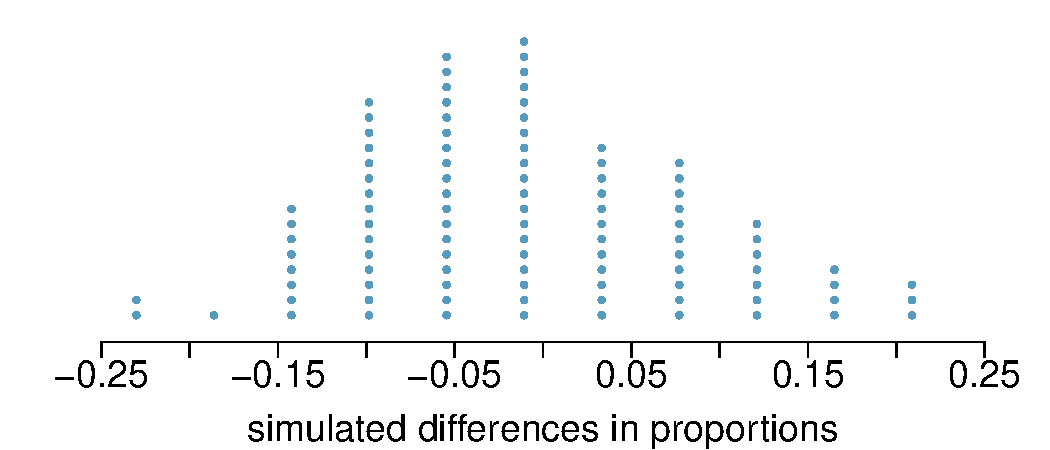
\includegraphics[width= 0.6\textwidth]{ch_summarizing_data/figures/eoce/randomization_heart_transplants/randomization_heart_transplants_rando.pdf}
\end{center}
}{}
